\section{Oracle APEX}

\subsection{Introduzione}
\textbf{Oracle APEX} (Application Express) è una piattaforma di sviluppo applicativo low-code che consente di creare applicazioni web scalabili, sicure e altamente performanti utilizzando il database Oracle come base.\\
Con Oracle APEX, è possibile sfruttare strumenti integrati per la creazione di interfacce utente, la gestione dei dati e la personalizzazione delle funzionalità, rendendo il processo di sviluppo rapido ed efficiente. È particolarmente utile per automatizzare processi aziendali, creare report interattivi e implementare soluzioni personalizzate su misura per le esigenze delle organizzazioni.

\subsection{Home}

\begin{figure}[ht!]
    \centering
    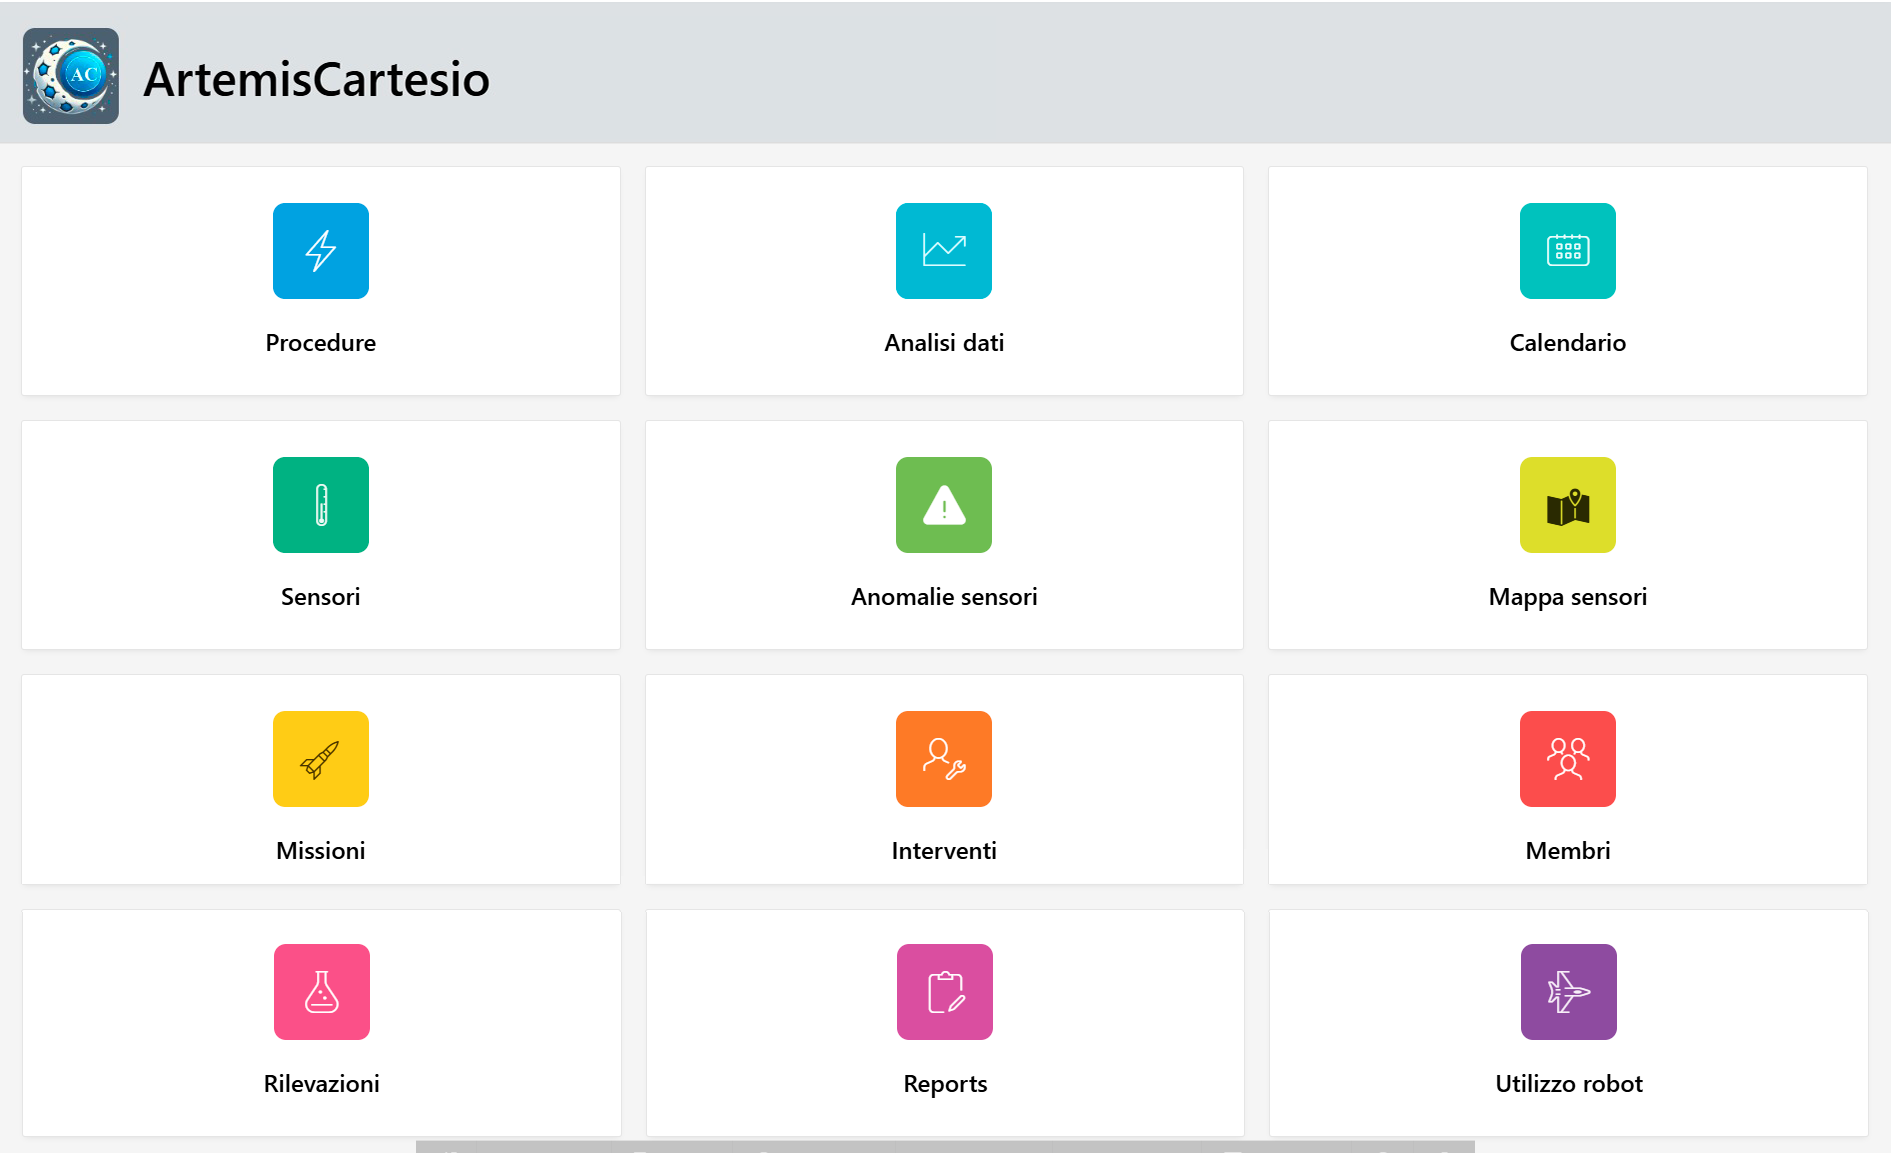
\includegraphics[width=\textwidth]{Media/App/home.png}
    \caption{Home page dell'applicazione}
    \label{fig:home_page}
\end{figure}

\noindent
In figura (Figura~\ref{fig:home_page}) è rappresentata la schermata principale dell'applicazione, progettata per gestire e monitorare ogni aspetto di una missione spaziale. La home page presenta una serie di funzionalità principali, ciascuna accessibile tramite icone intuitive e facilmente identificabili, che semplificano la navigazione e l'interazione con il sistema.\\
L'interfaccia è user-friendly e ben strutturata, progettata per garantire l'efficienza e la facilità d'uso per i membri dell'equipaggio della missione. Grazie all'organizzazione intuitiva, si può accedere rapidamente alle informazioni necessarie e ai moduli specifici per completare i propri compiti.

\subsection{Procedure}
\begin{figure}[ht!]
    \centering
    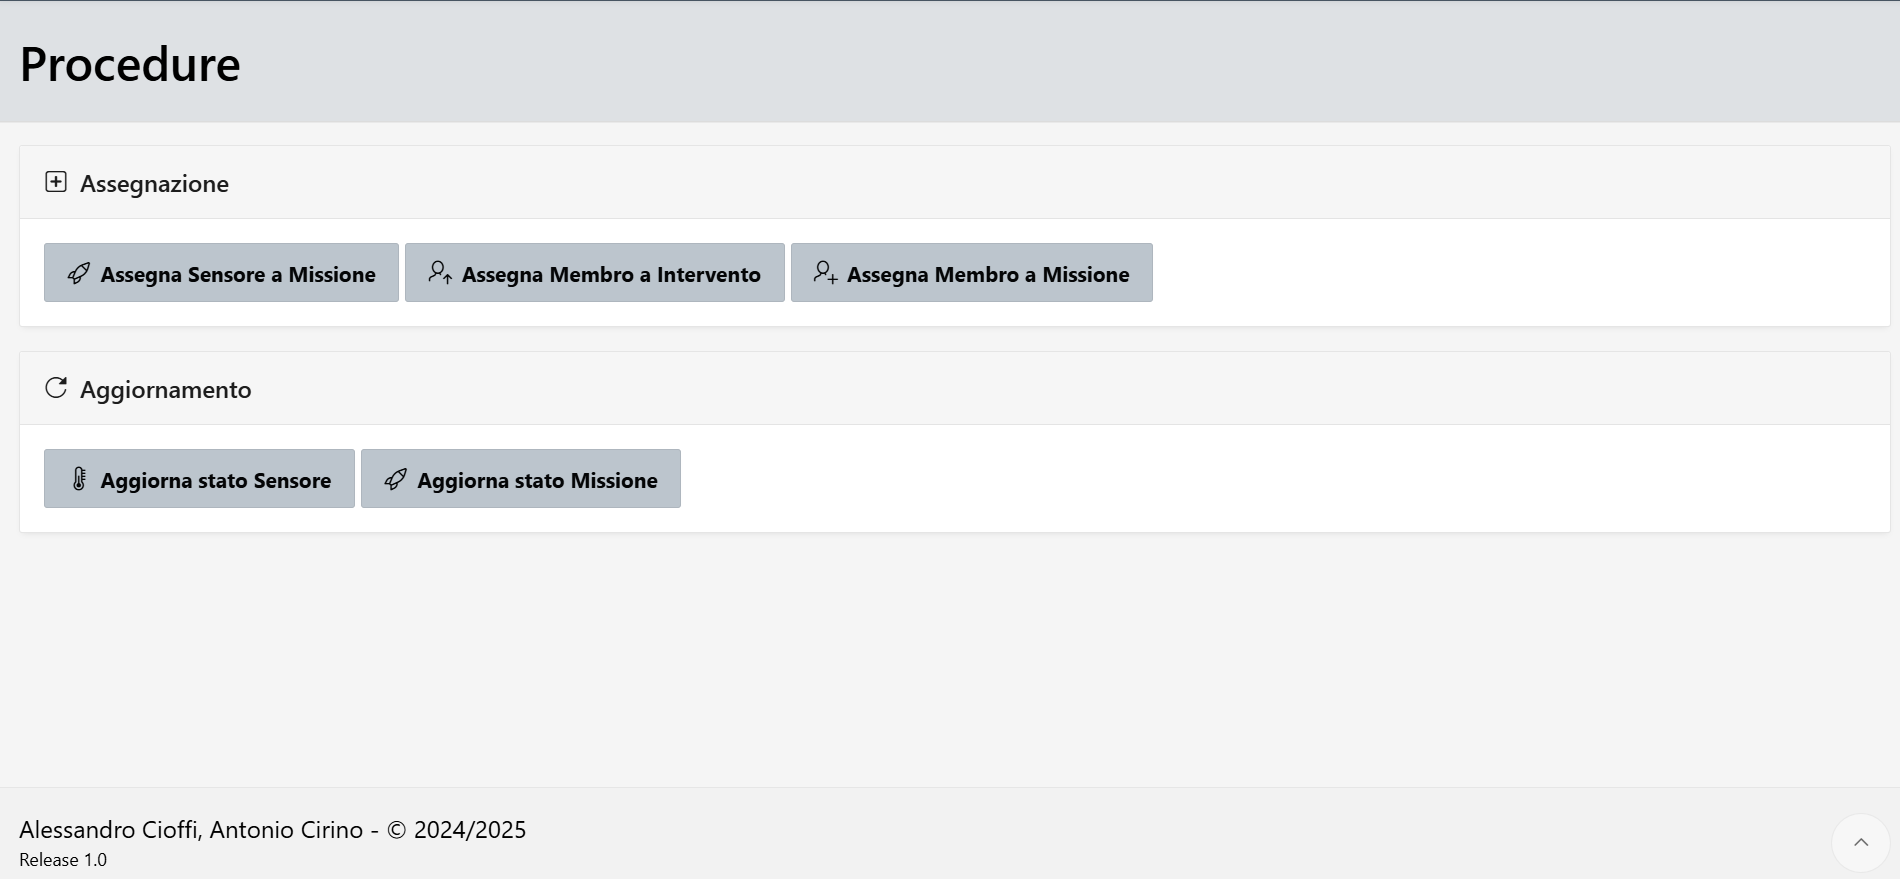
\includegraphics[width=\textwidth]{Media/App/procedure.png}
    \caption{Schermata della sezione \textit{Procedure}}
    \label{fig:procedure}
\end{figure}

\noindent
La schermata \textit{Procedure} è divisa in due sezioni: \textbf{Assegnazione} e \textbf{Aggiornamento}.

\paragraph{Assegnazione} Questa sezione permette di gestire l'allocazione delle risorse e del personale per le varie attività. Le funzionalità principali includono:
\begin{itemize}
    \item \textbf{Assegna Sensore a Missione}: consente di associare specifici sensori a una missione attiva.
    \item \textbf{Assegna Membro a Intervento}: permette di designare un membro del team per un determinato intervento tecnico (Figura~\ref{fig:procedura_assegnazione}).
    \item \textbf{Assegna Membro a Missione}: utilizzato per assegnare personale a una missione specifica.
\end{itemize}
\paragraph{Aggiornamento}
In questa sezione si possono effettuare aggiornamenti sullo stato dei sensori e delle missioni, garantendo che le informazioni siano sempre accurate e aggiornate. Le opzioni includono:
\begin{itemize}
    \item \textbf{Aggiorna stato Sensore}: modifica dello stato operativo di un sensore (attivo, malfunzionante, manutenzione, stand by) e della data dell'ultimo controllo (Figura~\ref{fig:procedura_aggiornamento}).
    \item \textbf{Aggiorna stato Missione}: consente di aggiornare lo stato di avanzamento di una missione (pianificata, in corso, completata, annullata).
\end{itemize}

\begin{figure}[ht!]
    \centering
    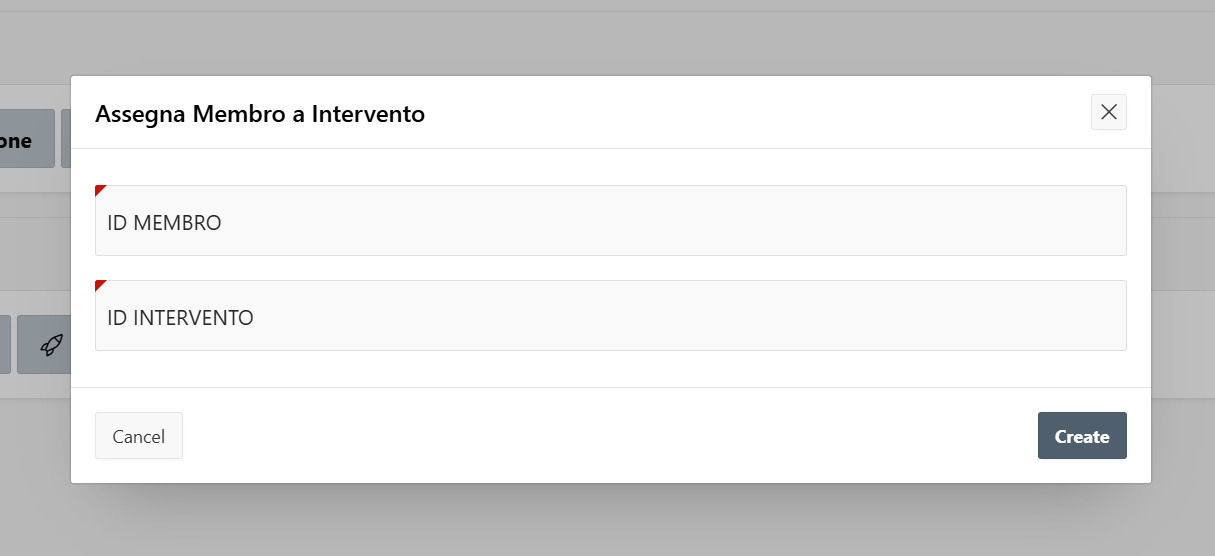
\includegraphics[width=0.8\textwidth]{Media/App/procedure_assegnazione.png}
    \caption{Finestra di dialogo per l'assegnazione di un membro ad un intervento}
    \label{fig:procedura_assegnazione}
\end{figure}

\begin{figure}[ht!]
    \centering
    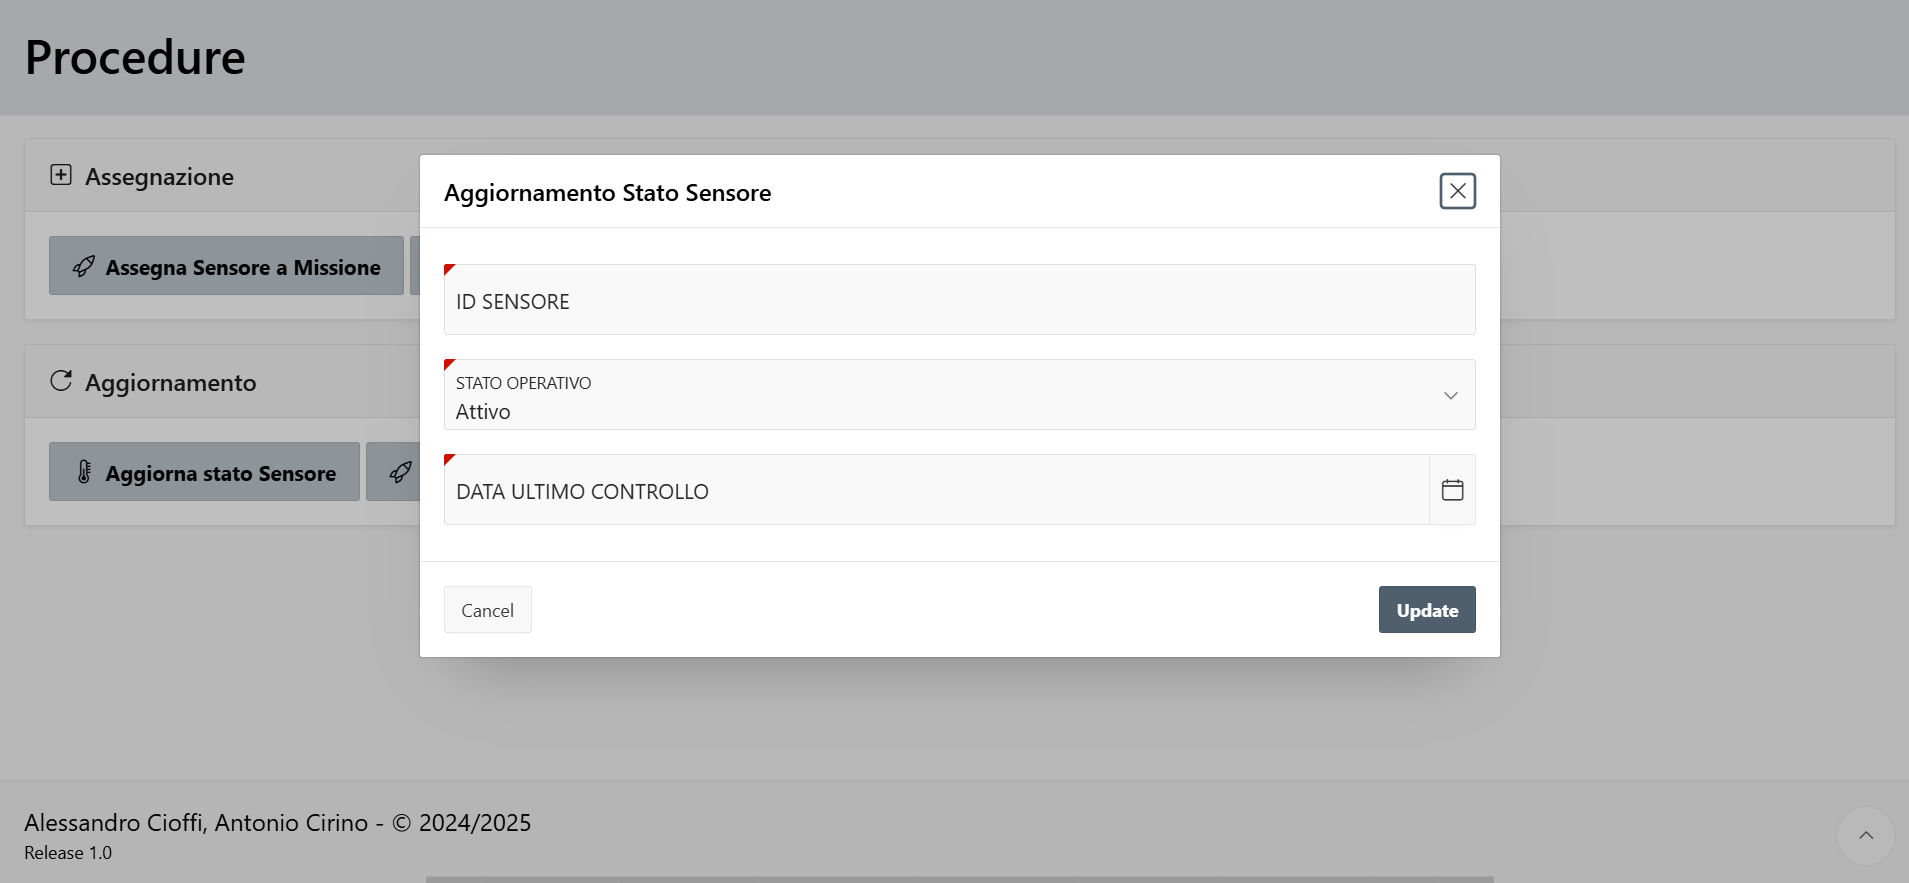
\includegraphics[width=0.8\textwidth]{Media/App/procedure_aggiornamento.png}
    \caption{Finestra di dialogo per l'aggiornamento di un sensore}
    \label{fig:procedura_aggiornamento}
\end{figure}


\subsection{Analisi dati}

\begin{figure}[ht!]
    \centering
    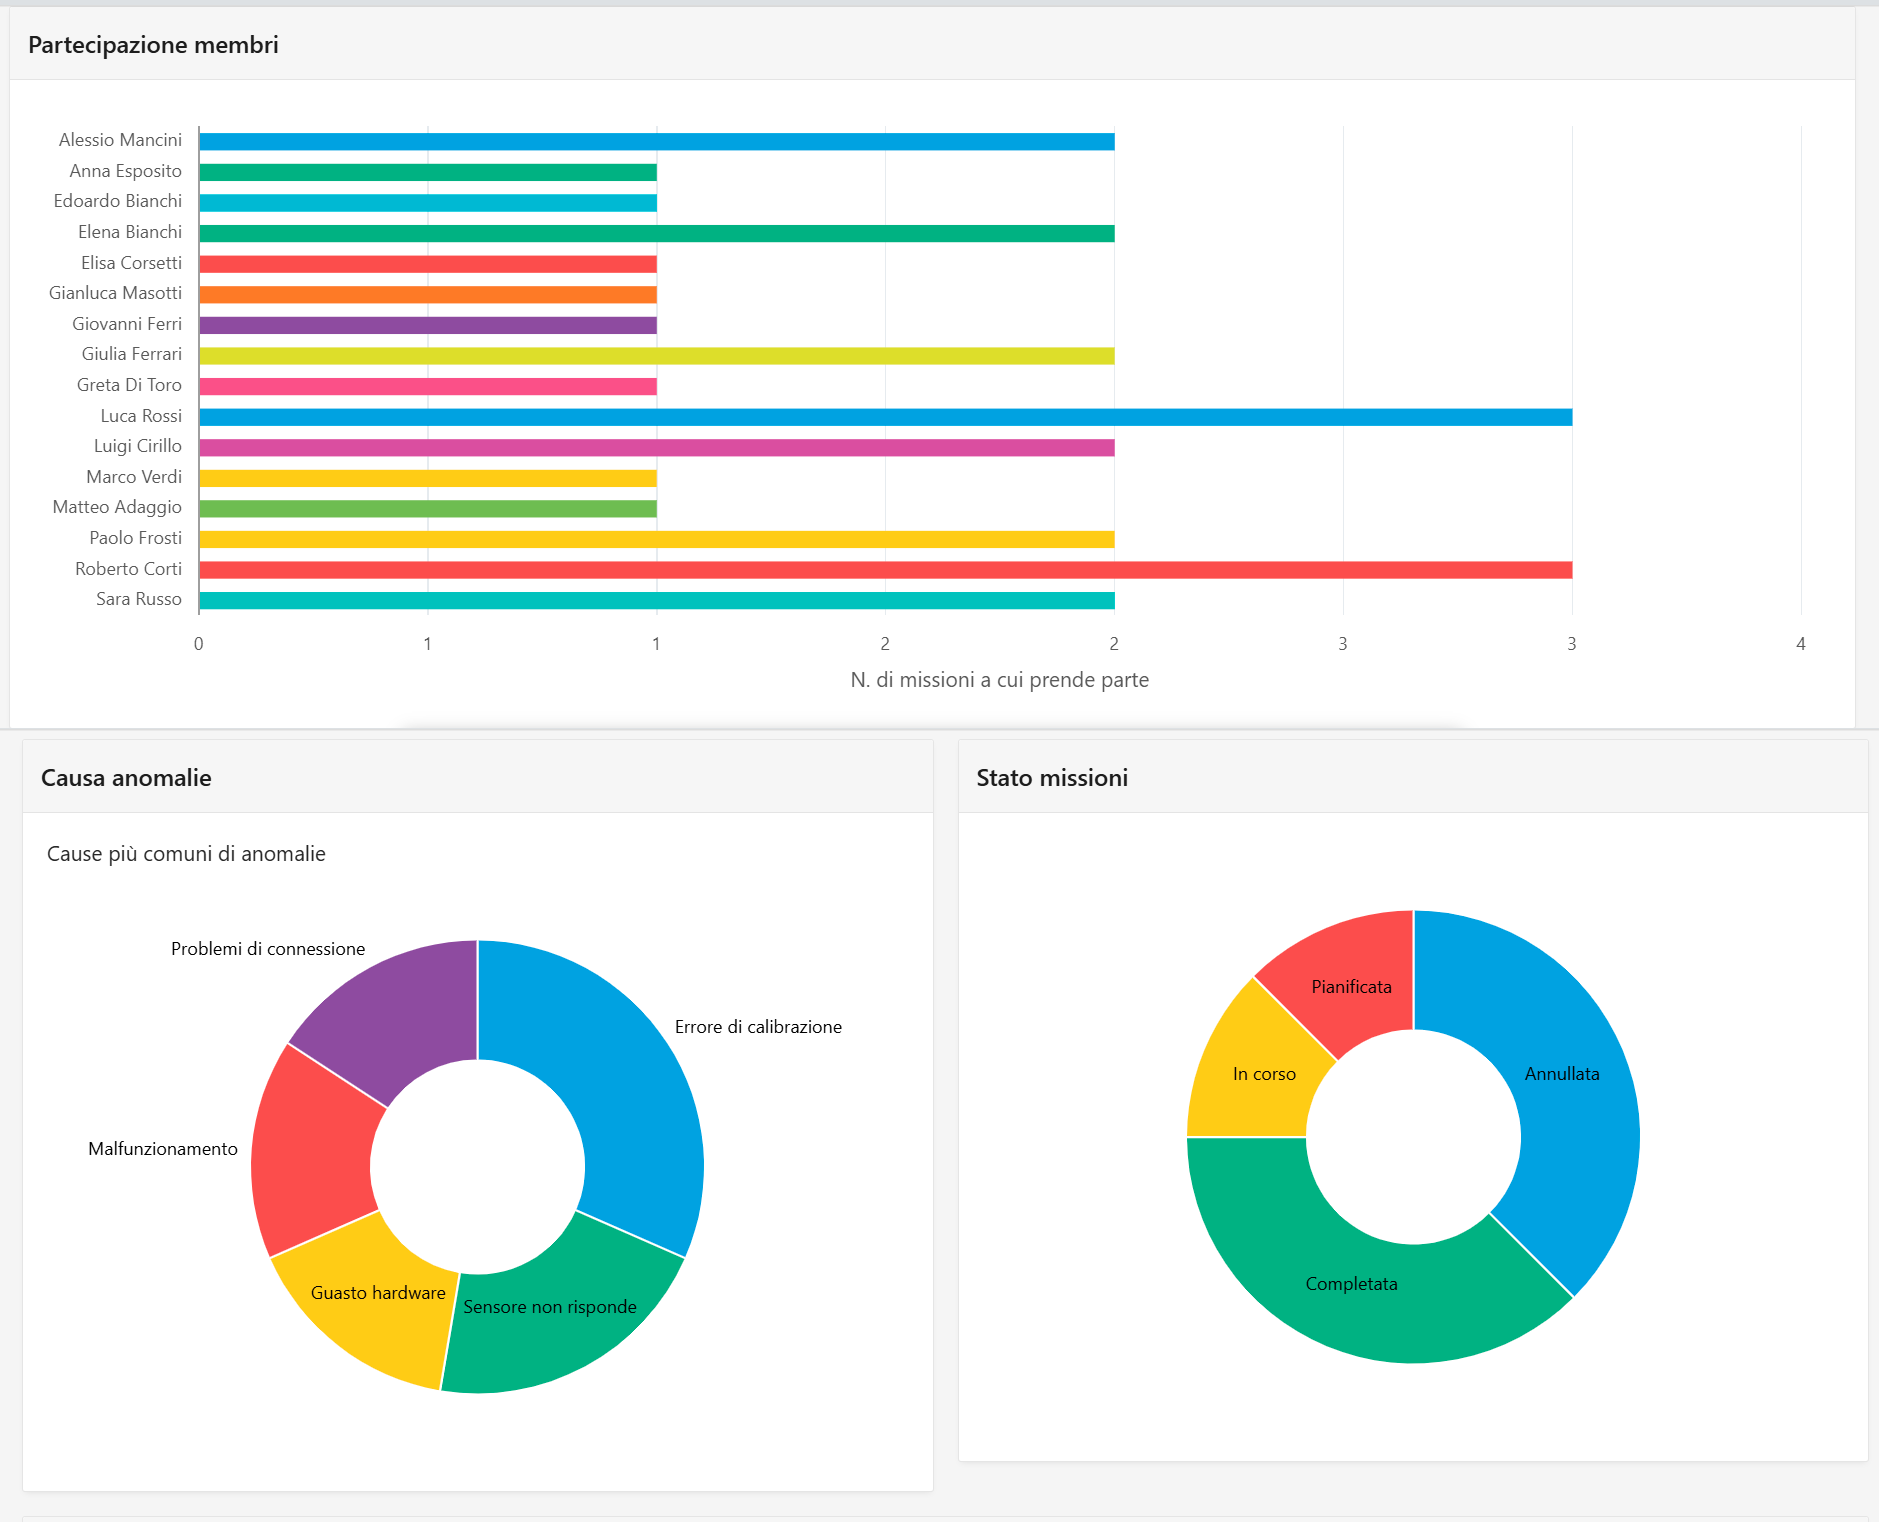
\includegraphics[width=\textwidth]{Media/App/analisi_dati.png}
    \caption{Schermata della sezione \textit{Analisi dati}}
    \label{fig:analisi_dati}
\end{figure}

L'immagine (Figura~\ref{fig:analisi_dati}) mostra la sezione \textbf{Analisi Dati} dell'applicazione ``Missione Lunare'', che fornisce una panoramica visiva sulle principali informazioni relative alla missione. La schermata include diversi grafici, tra cui:

\paragraph*{Partecipazione membri}
Un grafico a barre orizzontali che mostra il numero di missioni a cui ciascun membro del team partecipa. Questo consente di visualizzare rapidamente il grado di coinvolgimento dei membri nelle attività.

\paragraph{Causa anomalie}
Un grafico a ciambella che rappresenta le cause più comuni di anomalie registrate durante le missioni.

\paragraph*{Stato missioni}
Un secondo grafico a ciambella che evidenzia la distribuzione delle missioni in base al loro stato attuale. \\

\noindent
Questa sezione offre una visione chiara e intuitiva per monitorare il progresso e le criticità delle missioni, supportando un processo decisionale informato.


\subsection{Altre views}
Di seguito sono riportate altre sezioni presenti nell'applicazione:
\begin{figure}[ht!]
    \centering
    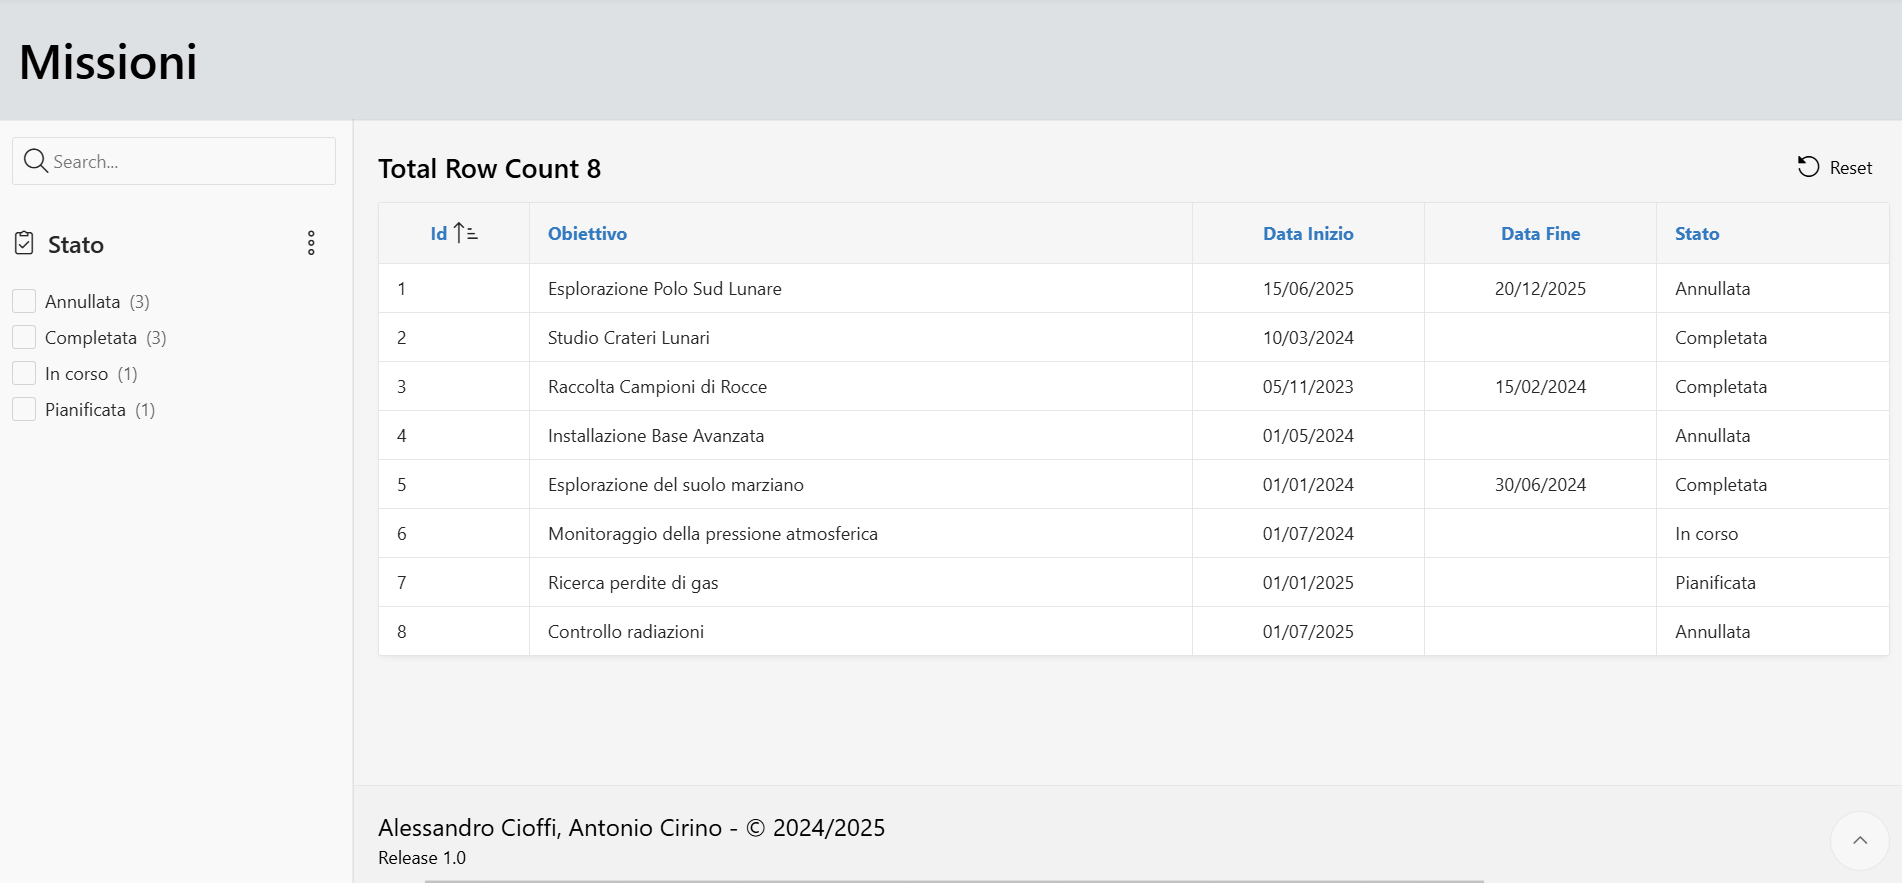
\includegraphics[width=0.9\textwidth]{Media/App/missioni.png}
    \caption{Schermata della sezione \textit{Missioni}}
    \label{fig:missioni}
\end{figure}
\begin{figure}[ht!]
    \centering
    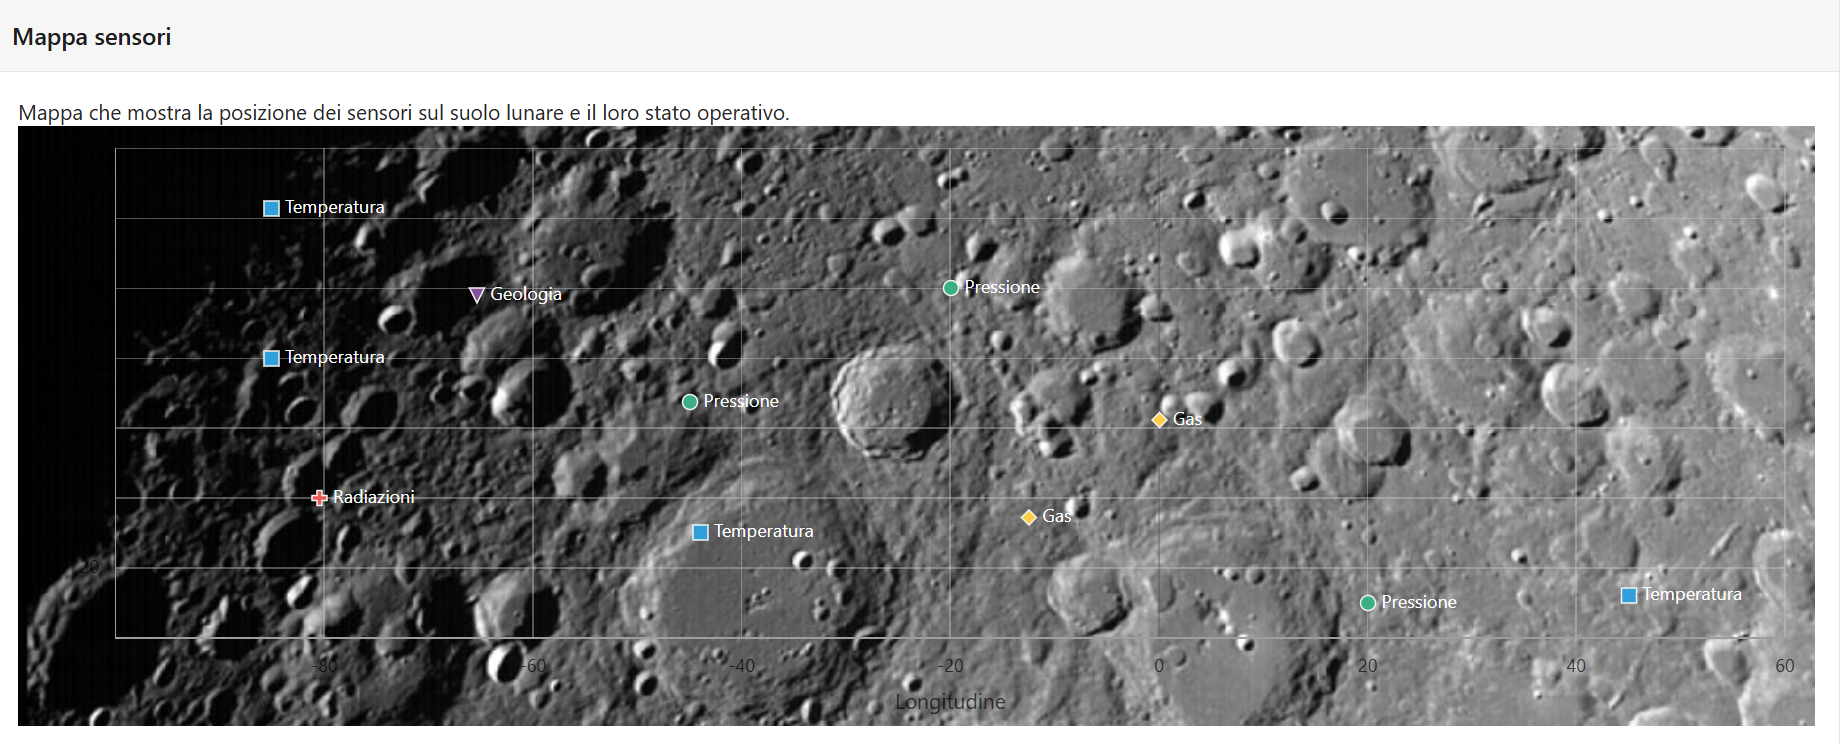
\includegraphics[width=0.9\textwidth]{Media/App/mappa_sensori.png}
    \caption{Schermata della sezione \textit{Mappa}}
    \label{fig:mappa}
\end{figure}
\begin{figure}[ht!]
    \centering
    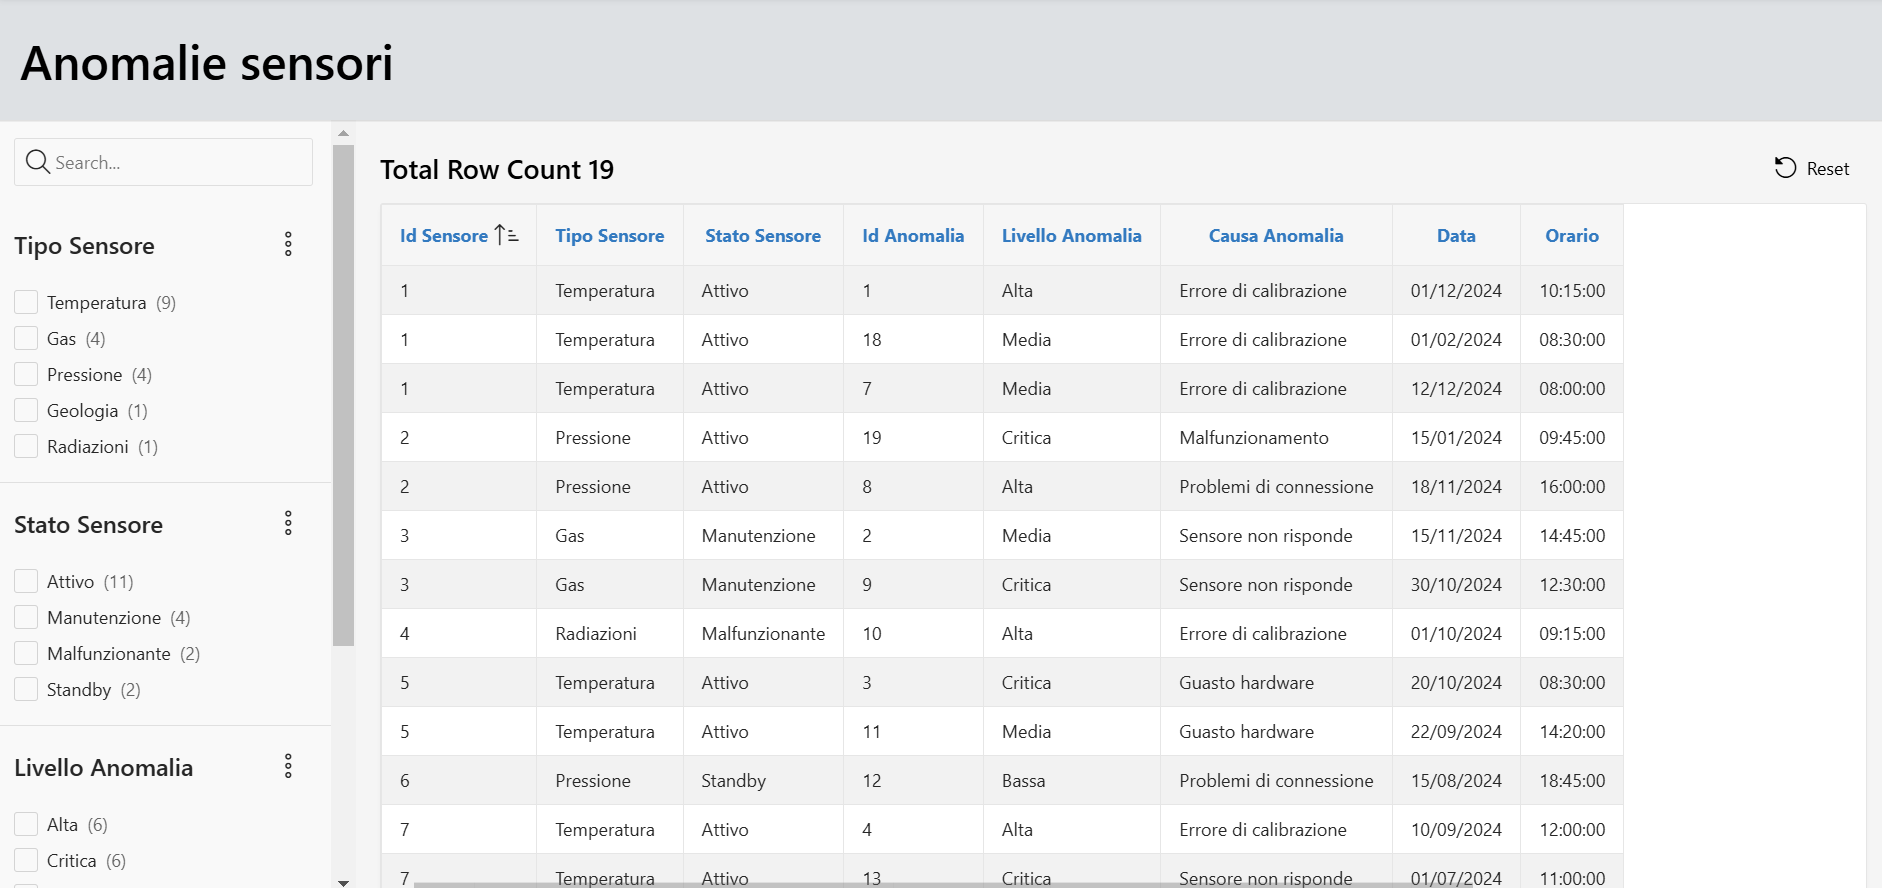
\includegraphics[width=0.9\textwidth]{Media/App/anomalie.png}
    \caption{Schermata della sezione \textit{Anomalie}}
    \label{fig:anomalie}
\end{figure}
\begin{figure}[ht!]
    \centering
    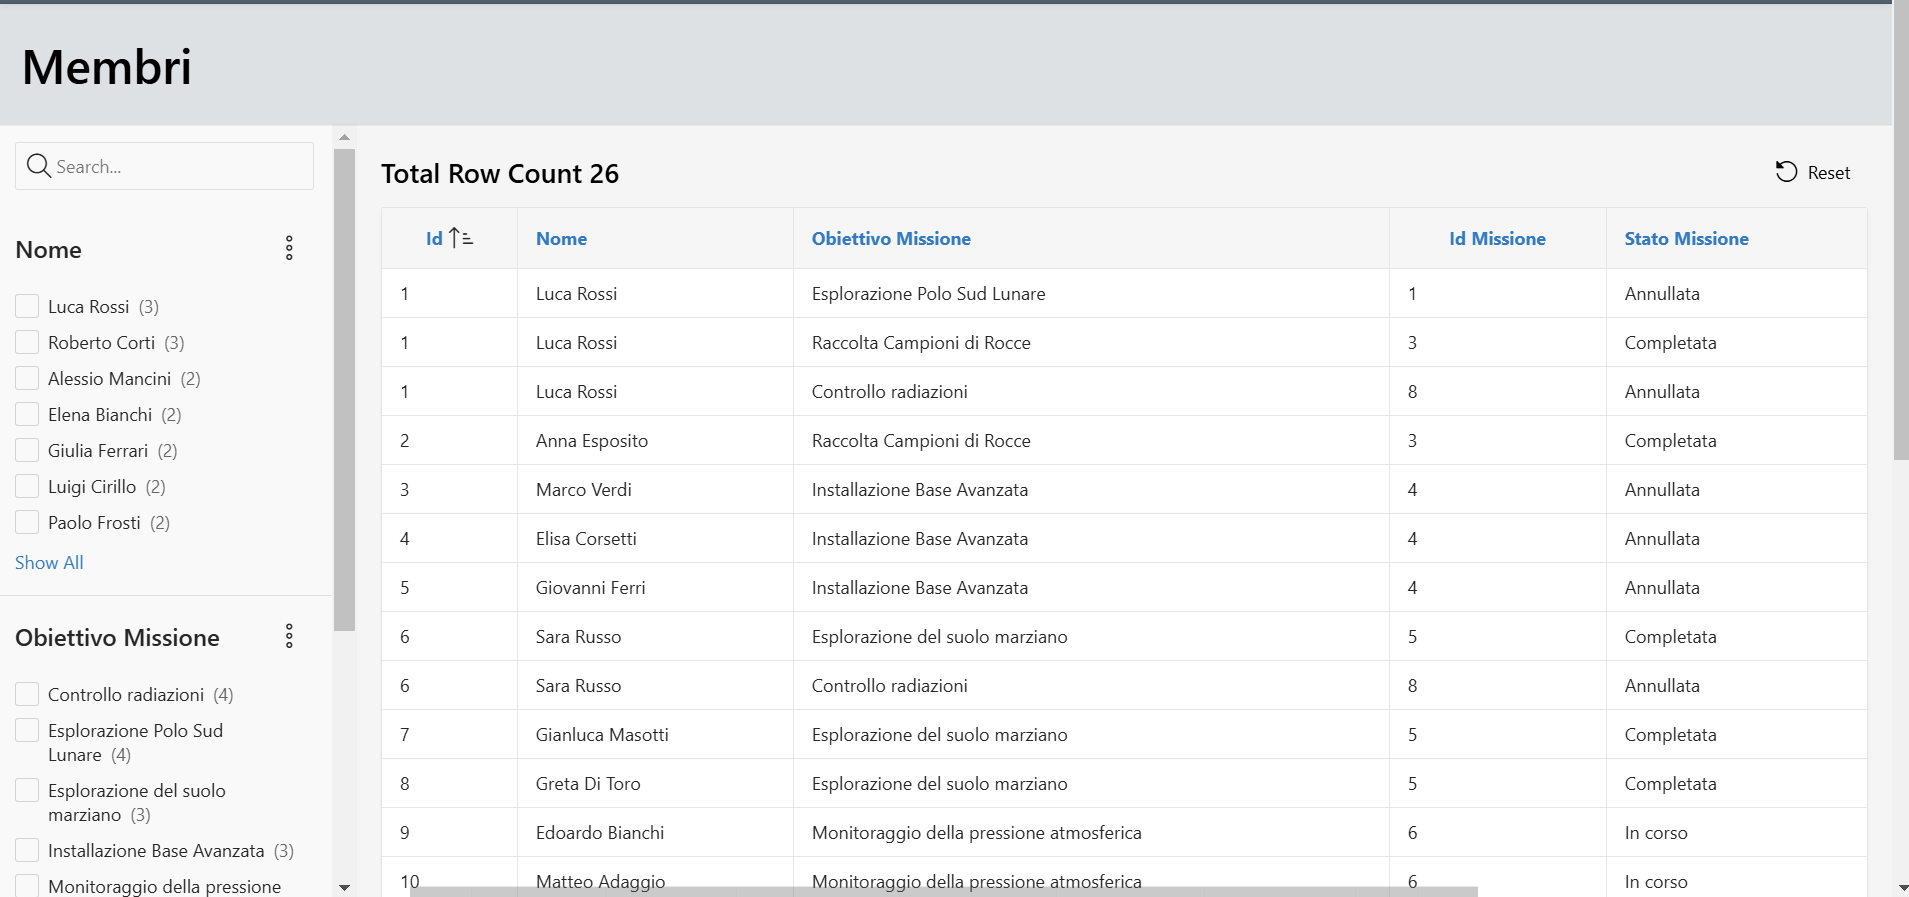
\includegraphics[width=0.9\textwidth]{Media/App/membri.png}
    \caption{Schermata della sezione \textit{Membri}}
    \label{fig:membri}
\end{figure}

\newpage
\subsection{Gestione della sicurezza}
Grazie alla sua profonda integrazione con il database Oracle, APEX garantisce sicurezza, affidabilità e un'elevata scalabilità, rendendolo ideale per progetti di qualsiasi dimensione, dalle piccole imprese alle grandi organizzazioni. \\

\begin{figure}[ht!]
    \centering
    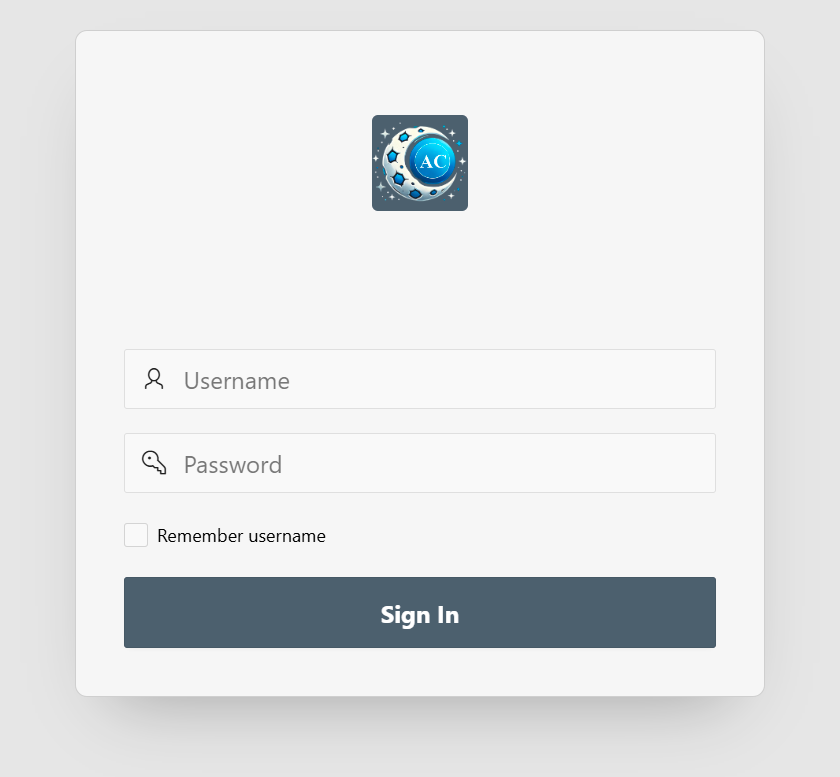
\includegraphics[width=0.5\textwidth]{Media/App/login.png}
    \caption{Schermata di login}
    \label{fig:login}
\end{figure}

\noindent
L'immagine (Figura~\ref{fig:login}) mostra la schermata di login dell'applicazione che implementa le best practice per garantire la sicurezza e la protezione dei dati. Questa schermata rappresenta il primo livello di sicurezza dell'applicazione, garantendo che solo utenti autorizzati possano accedere alle funzionalità e ai dati critici del sistema.
L'accesso all'applicazione è protetto da un sistema di login che richiede l'inserimento di username e password.\\
Oracle APEX utilizza inoltre meccanismi di crittografia per garantire la protezione delle credenziali durante la trasmissione dei dati e il sistema è progettato per prevenire vulnerabilità come SQL injection e brute force.




